\subsection{Event Selection Procedure}
\label{sec:selection}

Now that we have defined the signal we are searching for in ND280 and the reconstruction tools we have available, we develop a selection procedure to identify candidate $\nu_\mu$ charged current interactions. Primarily, we would like to identify the daughter muon produced by a $\nu_\mu$ charged current interaction $\nu_\mu + N \rightarrow \mu^- + X$ where X represents any particle or particles. This analysis uses neutrino events from the water-target region of the P0D where the daughter muon passes through the TPC. For the MC simulation, we use the NEUT generator. We use a cut-based selection technique and summarize the steps used:

\begin{itemize}
\item Data Quality Cuts.
\begin{enumerate}
	\item The data quality flag from the beam is good for the spill is ``good"
	\item The data quality flag from the near detector is also ``good"
\end{enumerate}
\item P0D to TPC1 Track Matching. Tracks are matched together using the algorithm described in Section \ref{sec:matching}.
\item Muon Tagging:
\begin{enumerate}
	\item Sort matched tracks by time stamp into 6 or 8 beam bunches depending on beam run.
	\item Evaluate the initial momentum of each matched track under a muon hypothesis. We use the Tracker measured momentum and correct for MIP-like energy loss in the P0D to evaluate the momentum. The exact method for this momentum calculation is described in Section \ref{sec:momrecon}.
	\item Select the highest momentum, negative track in each bunch in a fiducial volume slightly larger than nominal (FV+) as the muon candidate. The charge measurement comes from the Tracker. 
	\item Apply a nominal fiducial volume (FV) cut to the most upstream position of the P0D track requiring it to be within the official P0D water target fiducial volume. The volume boundaries of FV+ and FV are shown in Table \ref{tab:WTFV}.
\end{enumerate}
\end{itemize}

We also have an additional veto to filter out a specific type of background called ``sand muons". These backgrounds are discussed in great detail in Section \ref{sec:sandintsys}. Sand muons are negative MIP-like particles that are generated in the sand and concrete outside the ND280 and then pass through part of the detector. We also define negative MIP-like particles originating in the magnet yoke and the magnet coil as sand muons. These are clearly background as they are generated outside the fiducial volume, but they require special treatment. Since they are product of beam neutrino interactions, their timing structure mimics that of a signal event. They are also negative and MIP-like, so can easily be mistaken for a signal muon. Finally, sand muons are very poorly simulated, meaning that using MC to predict the sand muon background will not work. So we have found a way of achieving high sand muon exclusion rates by using the region of the P0D outside the fiducial volume to self-veto sand muon events.

\begin{itemize}
\item Sand Muon Veto:
\begin{enumerate}
	\item Count the number of external sand muon tracks entering the P0D. This is done by searching for Kalman fitted tracks in the P0D that begin outside the FV+ volume and end inside a similar volume that is slightly smaller in the Z-direction (FV-). The volume boundaries of FV- is shown in Table \ref{tab:WTFV}.
	\item If there is a concurrent sand muon in the same bunch as a candidate muon track, we veto the entire bunch. This accounts for possible reconstruction failures where a broken sand muon track is identified as a potential muon track beginning in the nominal FV. This is shown in Figure \ref{fig:smveto}.
\end{enumerate}
\end{itemize}

\begin{table}[h]
\caption{The P0D Water-Target Fiducial Volumes used in this analysis. The nominal fiducial volume cut (FV) is applied to all events. The other two volumes (FV+) and (FV-) are used in the process of selection. All units are in mm.}
\centering
\begin{tabular}{ccccccc}
\toprule
Axis & FV (min) & FV (max) & FV+ (min) & FV+ (max) & FV- (min) & FV- (max) \\
\hline
X & -836 & 764 & -988 & 910 & -988 & 910\\
Y & -871 & 869 & -1020 & 1010 & -1020 & 1010\\
Z & -2969 & -1264 & -3139 & -900 & -3139 & -987\\
\bottomrule
\end{tabular} 
\label{tab:WTFV} 
\end{table}

\begin{figure}[h]
\centering
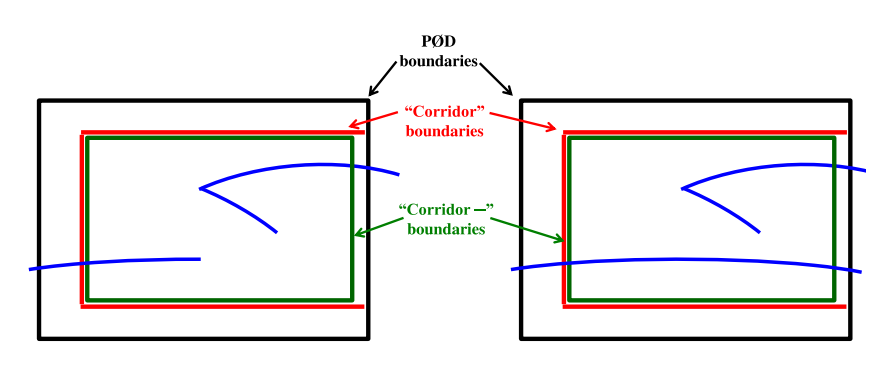
\includegraphics[width=6in]{Figures/smveto.png}
\caption{Graphic showing the two fiducial volume cuts used to veto sand muons. The ``Corridor" (red) boundary is the FV+ volume and the ``Corridor-" (green) boundary is the FV- volume. The external, entering sand muon track that stops in the P0D (left) causes a veto of a candidate CC inclusive event. The external, passing through sand muon track (right) does not cause a veto.}
\label{fig:smveto}
\end{figure}


\subsection{Event Selection Results}
\label{sec:selresults}

The results of the selection and the event reduction are plotted for different runs in Figures \ref{fig:xs1run1water} to \ref{fig:xs2run4air}. We also include the signal efficiency as a function of each variable. The efficiency is calculated as
\begin{equation}
\epsilon = \frac{\text{\# selected signal evts.}}{\text{\# total signal evts}}.
\end{equation}
\noindent We expect the total signal event rates to not vary as a function of the XY vertex position, so it is sensible that the signal efficiency shape mimics the event rate distribution. To first order, the data and MC reasonably track one another in the 1-D vertex distributions, though there is a discrepancy in the overall normalization. The momentum and theta distributions are a lot more interesting as they show very clearly the limitations of this selection. Specifically, we are sensitive to the higher momentum, forward-going muons and lose a lot of the steeper, low-energy muon tracks. 

\begin{figure}[h]
\centering
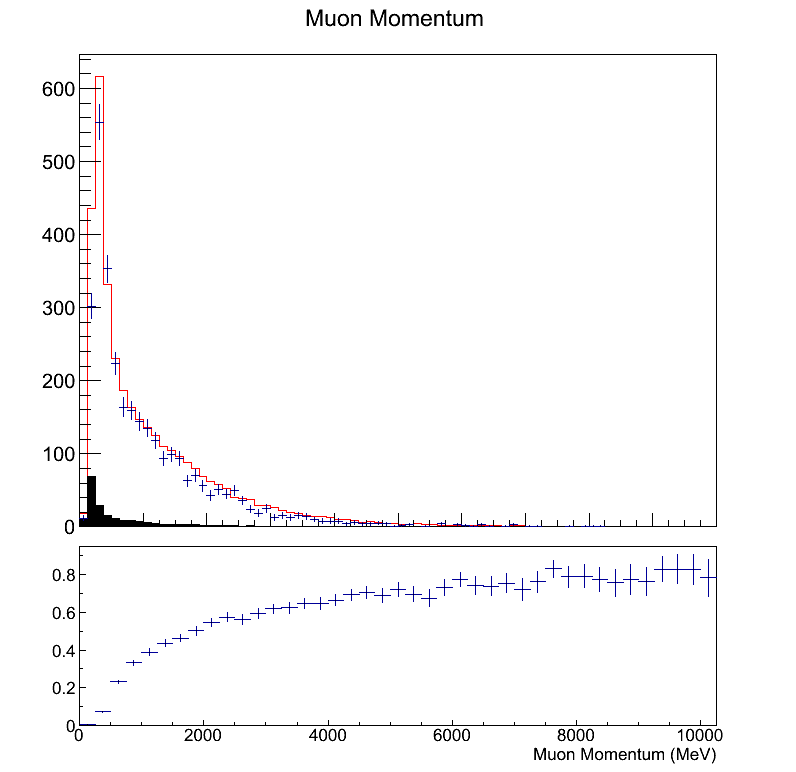
\includegraphics[width=3in]{Figures/TN100Plots/c_Pwater_1.png}
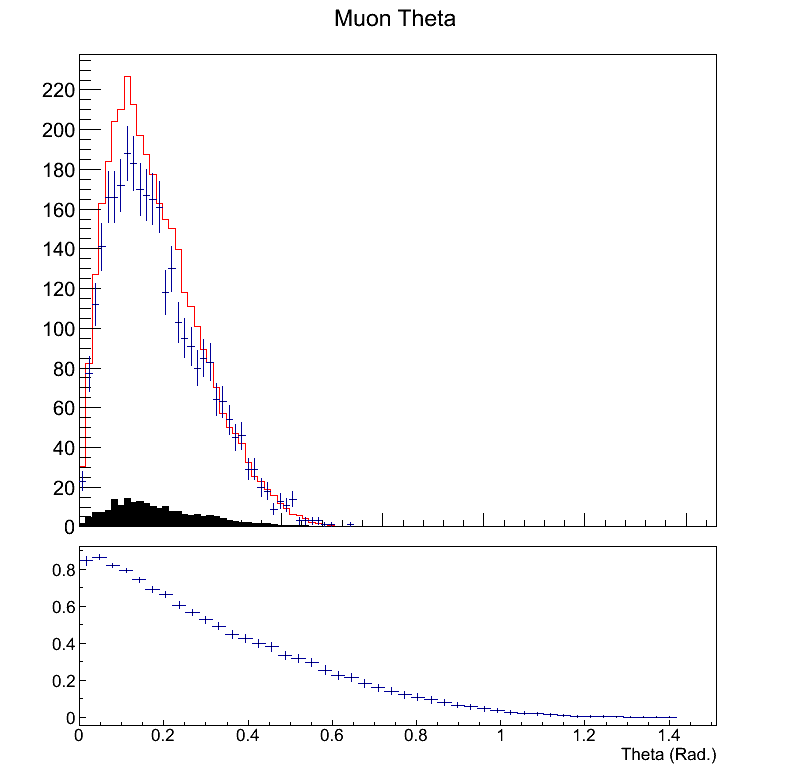
\includegraphics[width=3in]{Figures/TN100Plots/c_Thwater_1.png}
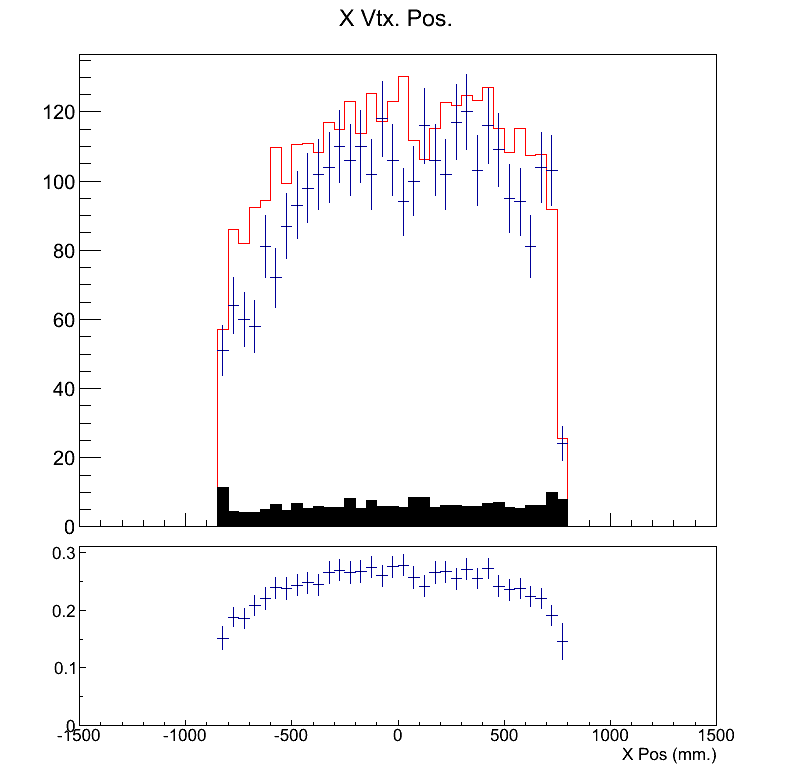
\includegraphics[width=3in]{Figures/TN100Plots/c_Xwater_1.png}
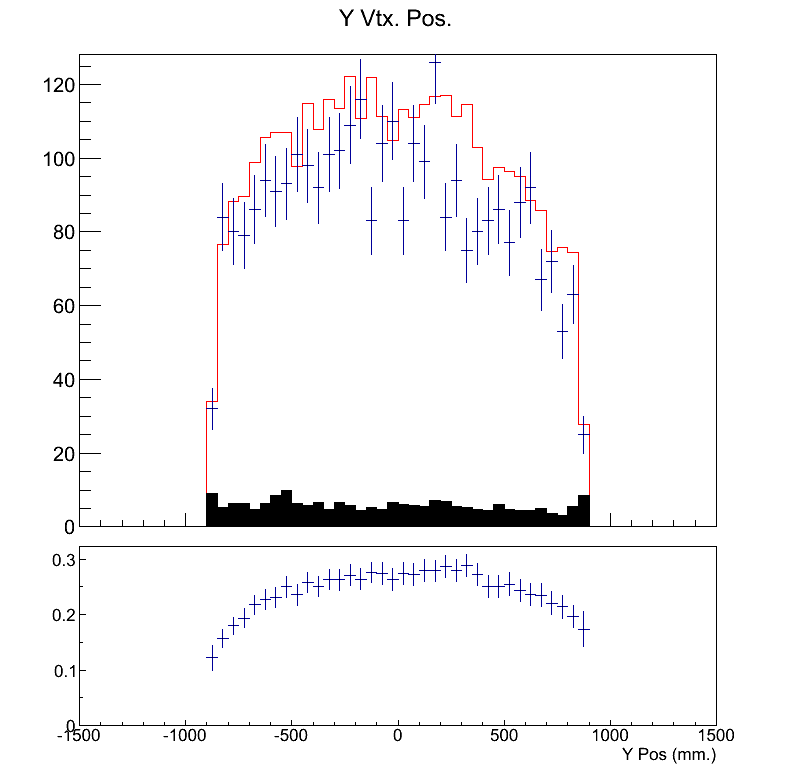
\includegraphics[width=3in]{Figures/TN100Plots/c_Ywater_1.png}
\caption{Kinematic and Vertex position distributions for selected events in run 1 water-in data. The data with error is shown with blue crosses and the MC signal and background are shown in red and black respectively. Below each distribution histogram is the MC predicted signal efficiency as a function of the same variable.}
\label{fig:xs1run1water}
\end{figure}

\begin{figure}[h]
\centering
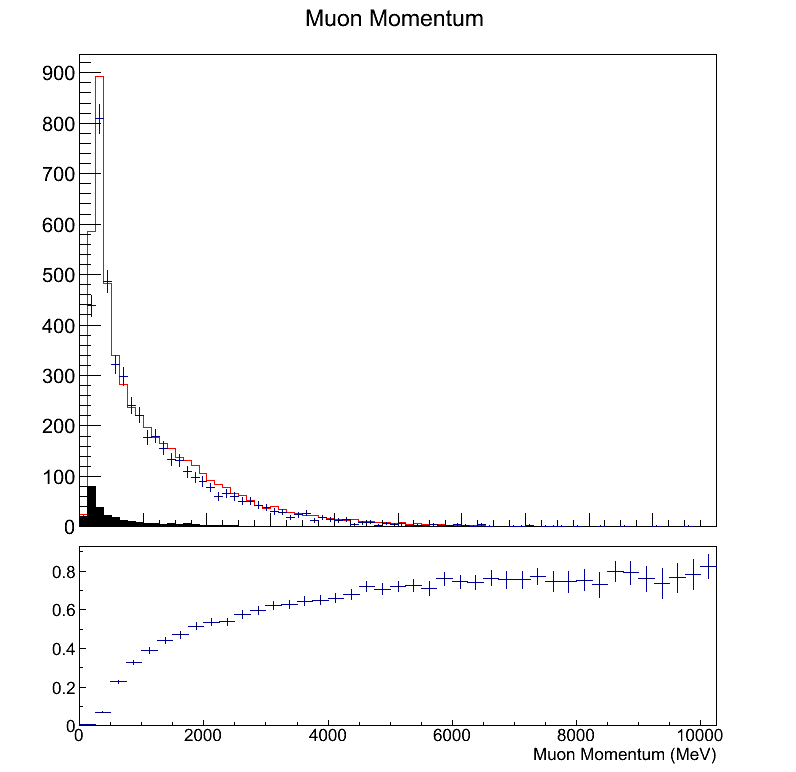
\includegraphics[width=3in]{Figures/TN100Plots/c_Pwater_2.png}
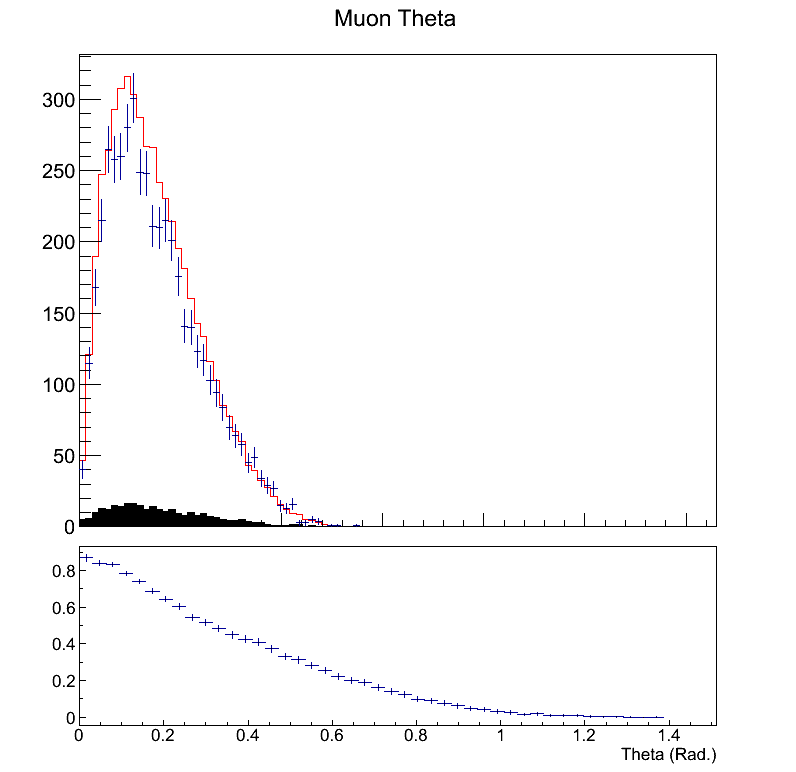
\includegraphics[width=3in]{Figures/TN100Plots/c_Thwater_2.png}
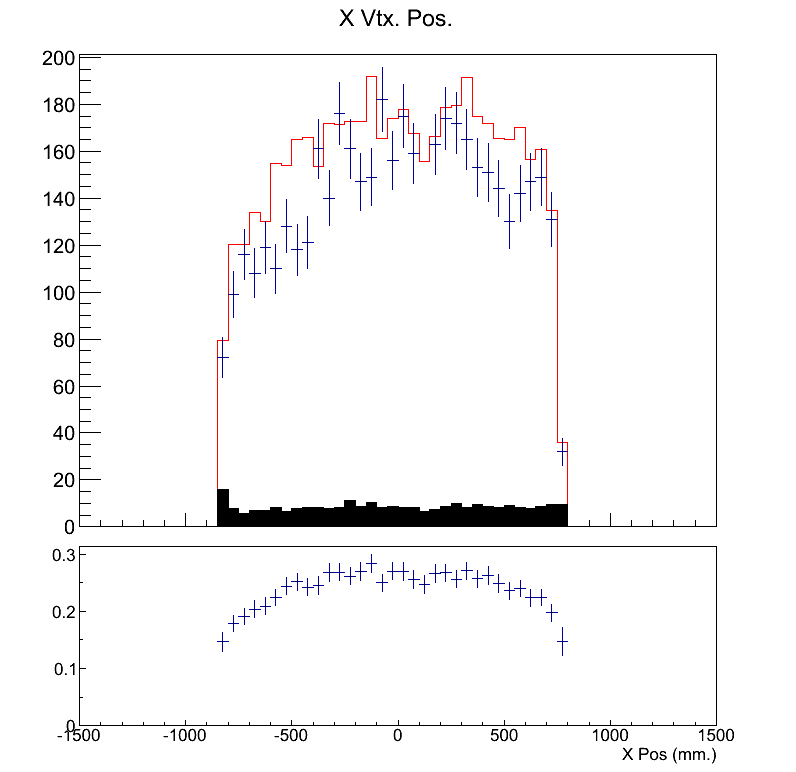
\includegraphics[width=3in]{Figures/TN100Plots/c_Xwater_2.png}
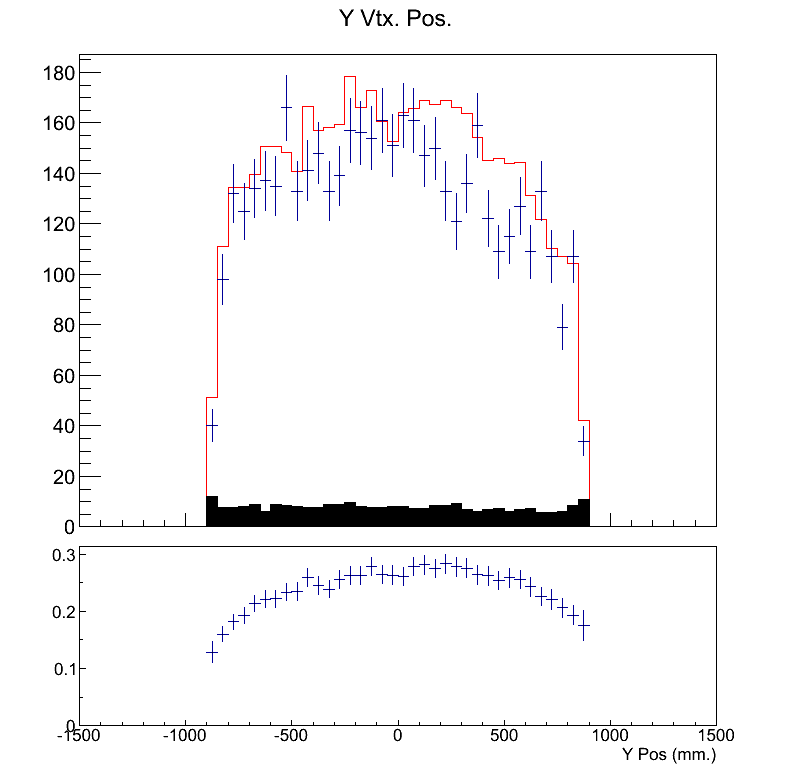
\includegraphics[width=3in]{Figures/TN100Plots/c_Ywater_2.png}
\caption{Kinematic and Vertex position distributions for selected events in run 2 water-in.  The data with error is shown with blue crosses and the MC signal and background are shown in red and black respectively. Below each distribution histogram is the MC predicted signal efficiency as a function of the same variable.}
\label{fig:xs1run2water}
\end{figure}

\begin{figure}[h]
\centering
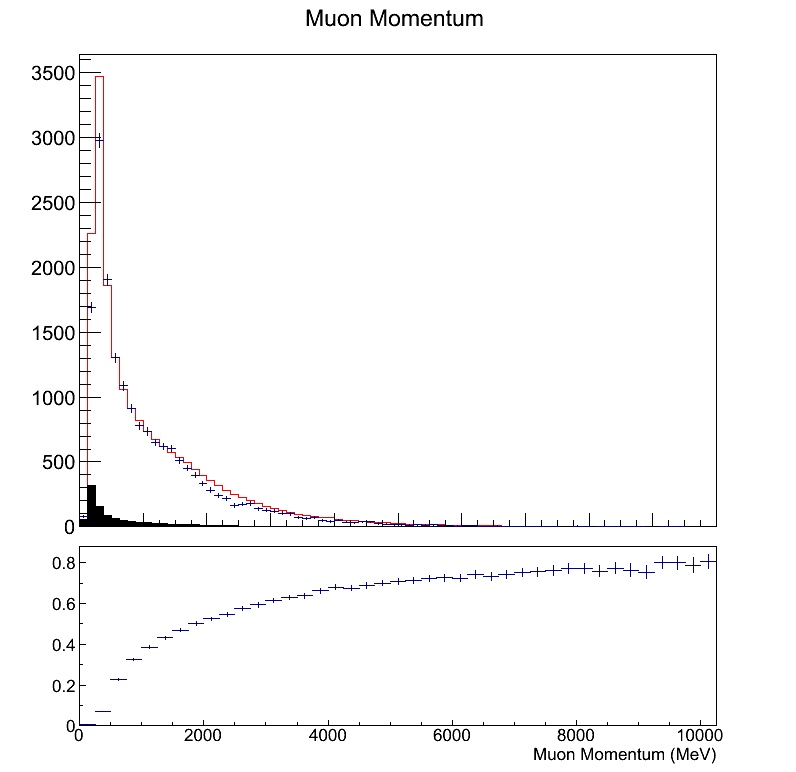
\includegraphics[width=3in]{Figures/TN100Plots/c_Pwater_4.png}
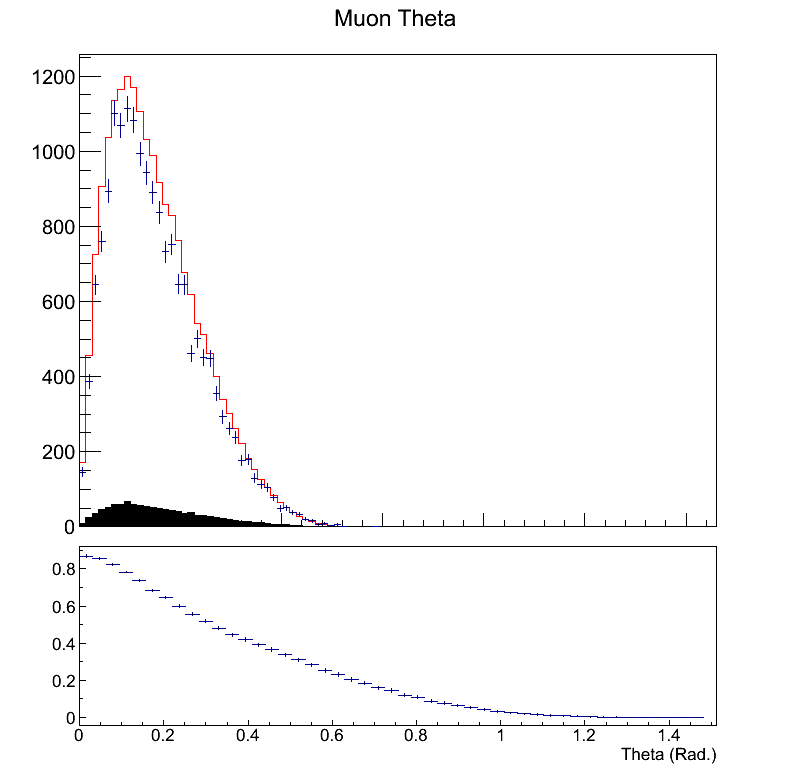
\includegraphics[width=3in]{Figures/TN100Plots/c_Thwater_4.png}
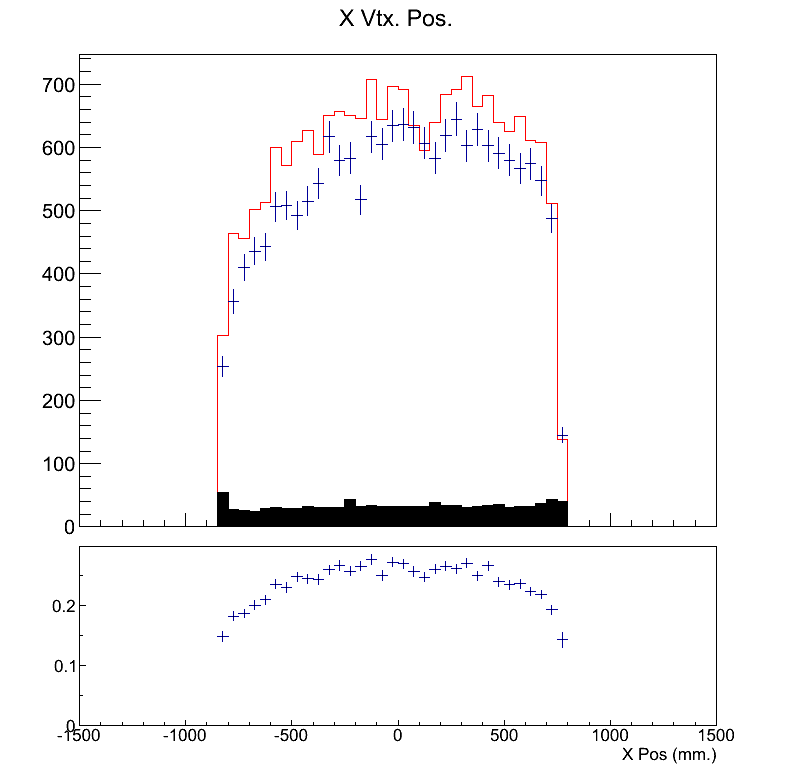
\includegraphics[width=3in]{Figures/TN100Plots/c_Xwater_4.png}
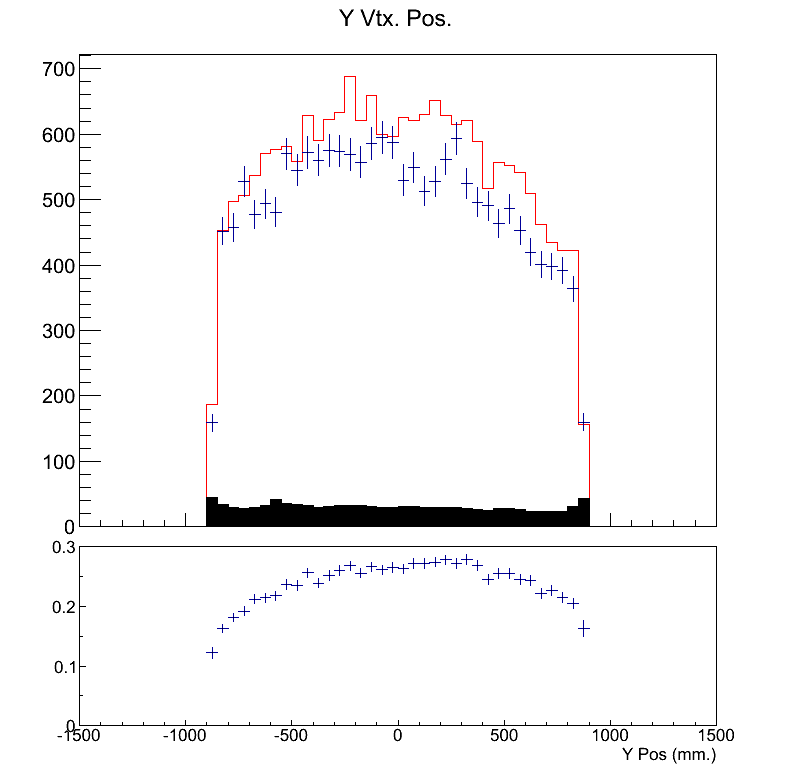
\includegraphics[width=3in]{Figures/TN100Plots/c_Ywater_4.png}
\caption{Kinematic and Vertex position distributions for selected events in run 4 water-in.  The data with error is shown with blue crosses and the MC signal and background are shown in red and black respectively. Below each distribution histogram is the MC predicted signal efficiency as a function of the same variable.}
\label{fig:xs1run4water}
\end{figure}

\begin{figure}[h]
\centering
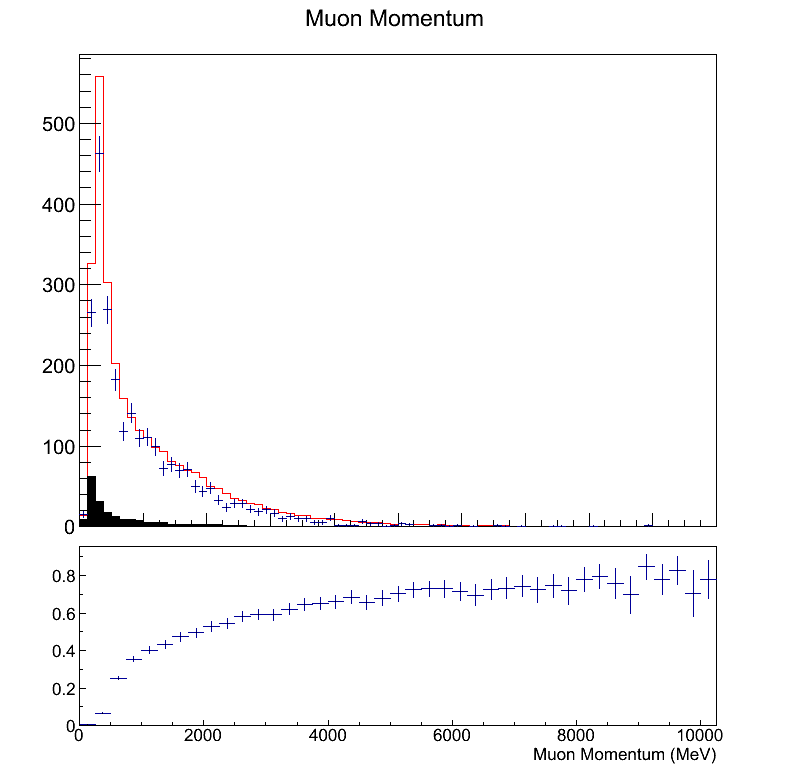
\includegraphics[width=3in]{Figures/TN100Plots/c_Pair_2.png}
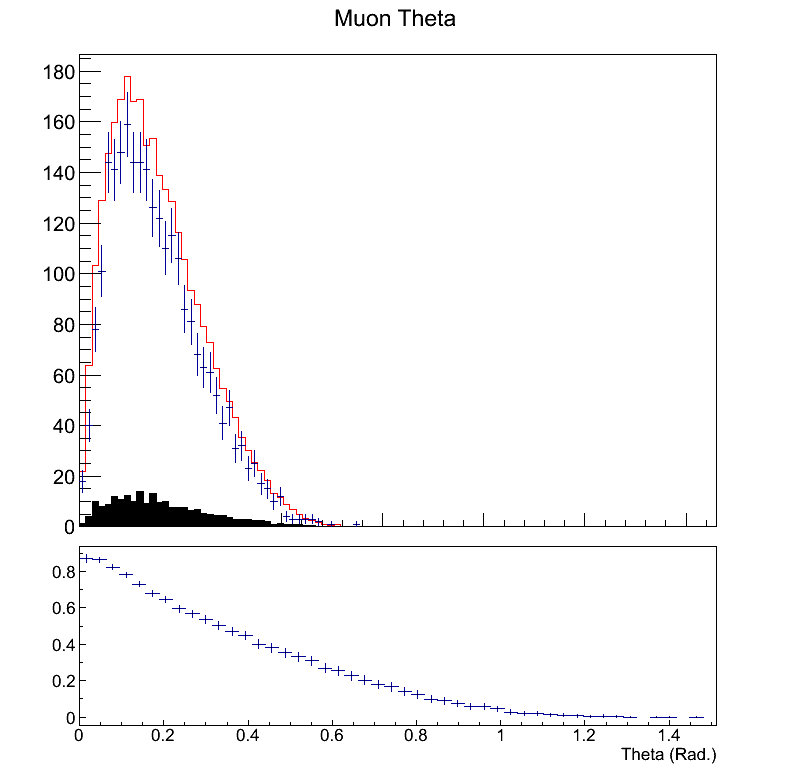
\includegraphics[width=3in]{Figures/TN100Plots/c_Thair_2.png}
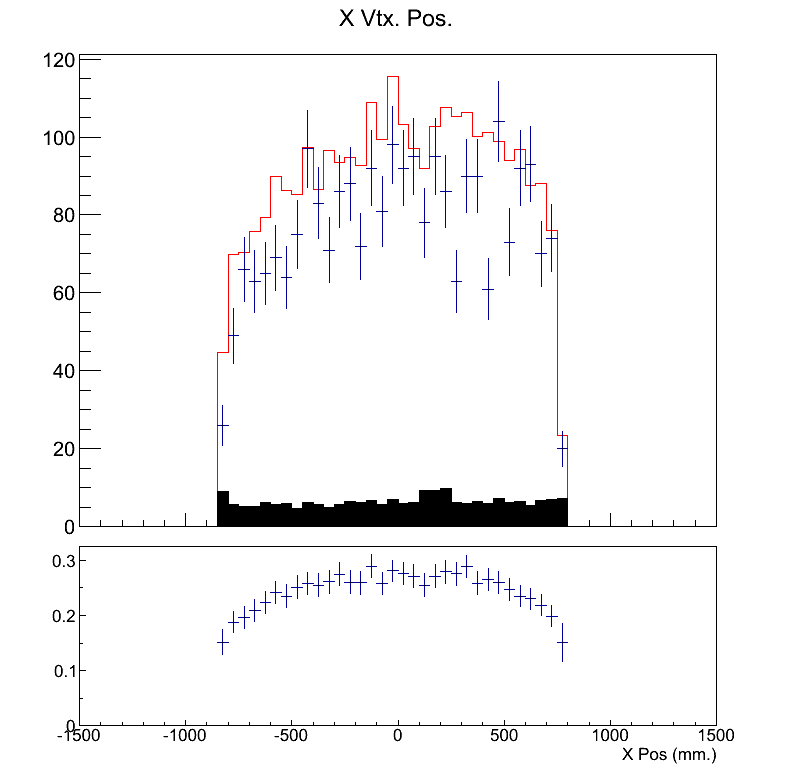
\includegraphics[width=3in]{Figures/TN100Plots/c_Xair_2.png}
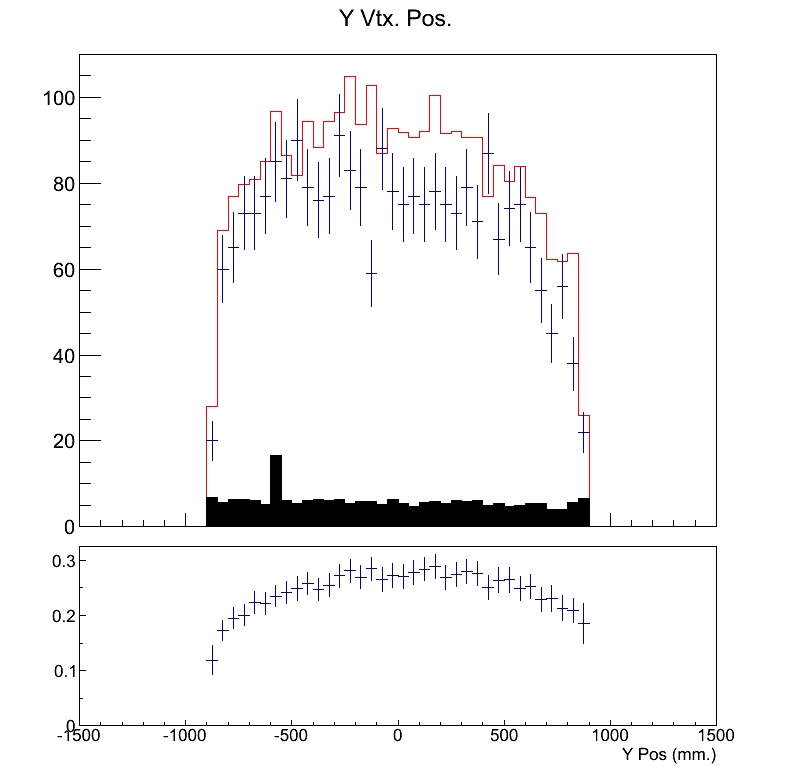
\includegraphics[width=3in]{Figures/TN100Plots/c_Yair_2.png}
\caption{Kinematic and Vertex position distributions for selected events in run 2 water-out. The data with error is shown with blue crosses and the MC signal and background are shown in red and black respectively.  Below each distribution histogram is the MC predicted signal efficiency as a function of the same variable.}
\label{fig:xs2run2air}
\end{figure}

\begin{figure}[h]
\centering
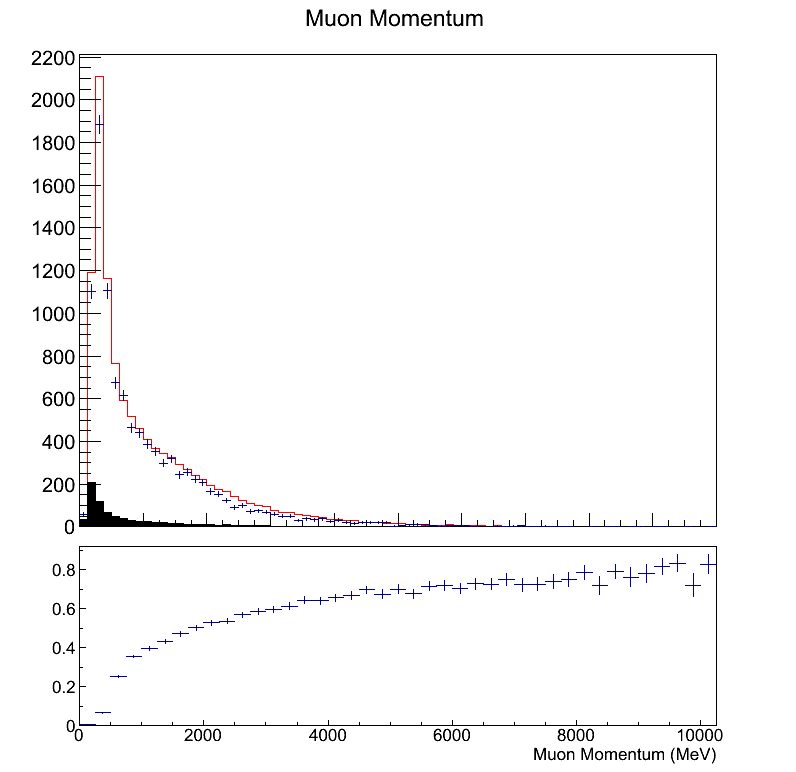
\includegraphics[width=3in]{Figures/TN100Plots/c_Pair_3.png}
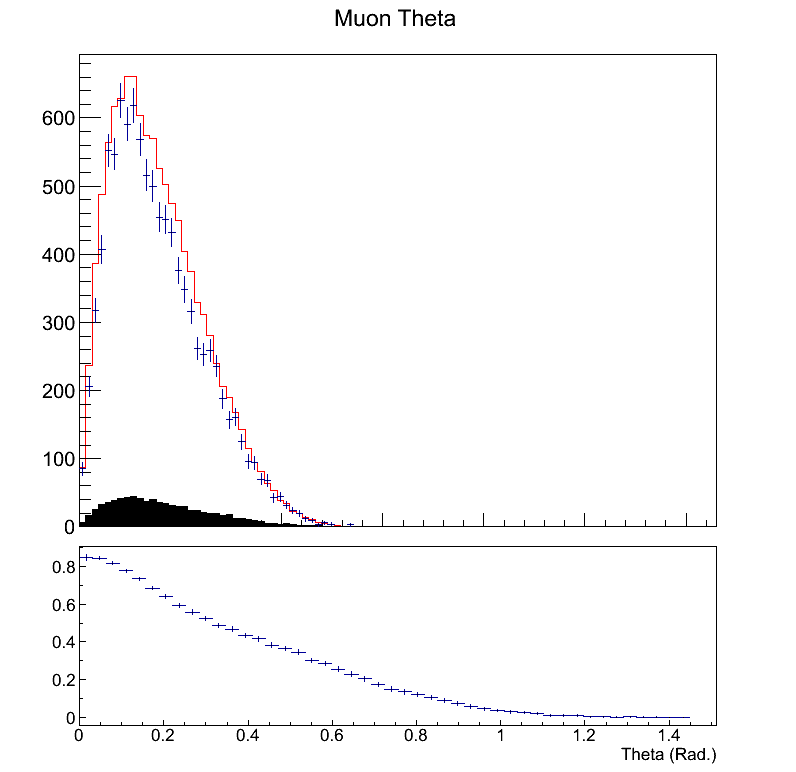
\includegraphics[width=3in]{Figures/TN100Plots/c_Thair_3.png}
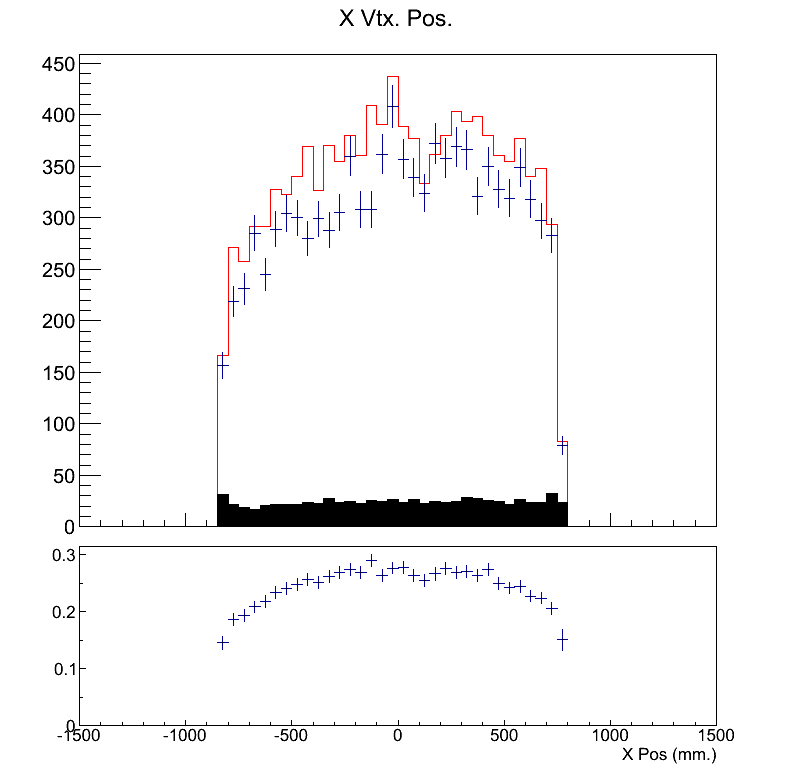
\includegraphics[width=3in]{Figures/TN100Plots/c_Xair_3.png}
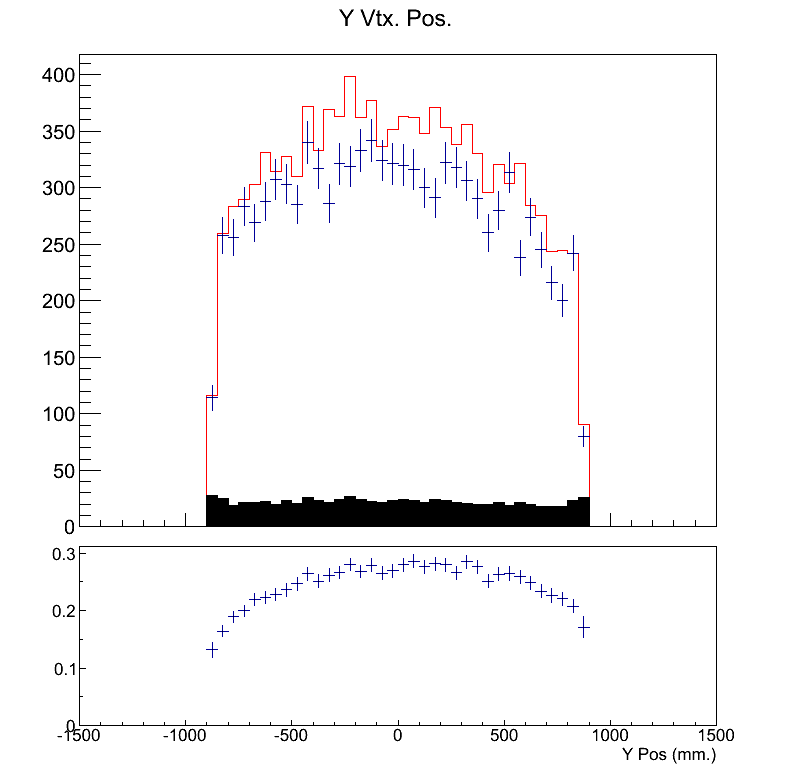
\includegraphics[width=3in]{Figures/TN100Plots/c_Yair_3.png}
\caption{Kinematic and Vertex position distributions for selected events in run 3 water-out. The data with error is shown with blue crosses and the MC signal and background are shown in red and black respectively. Below each distribution histogram is the MC predicted signal efficiency as a function of the same variable.}
\label{fig:xs2run3air}
\end{figure}

\begin{figure}[h]
\centering
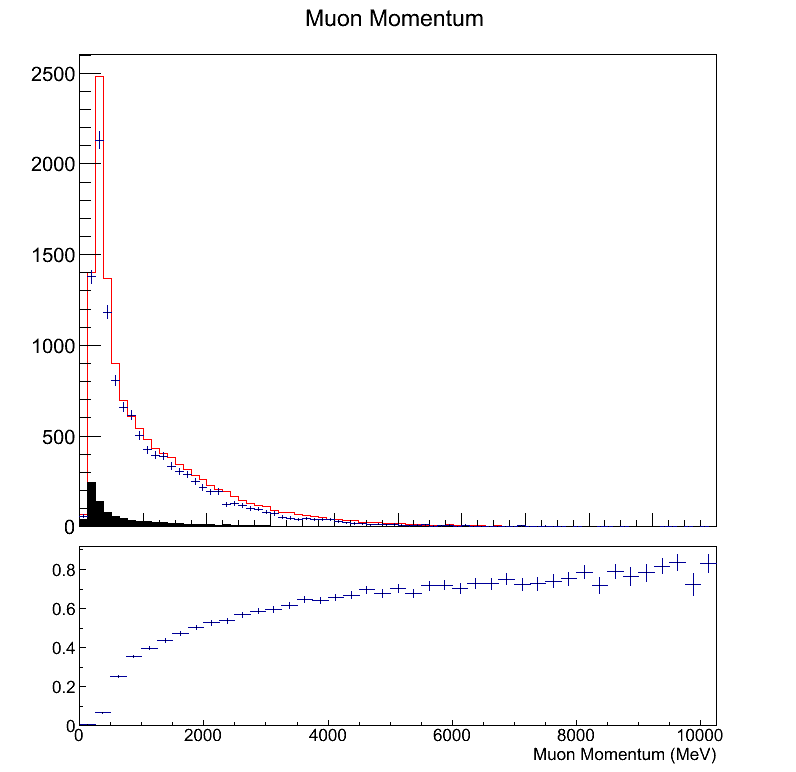
\includegraphics[width=3in]{Figures/TN100Plots/c_Pair_4.png}
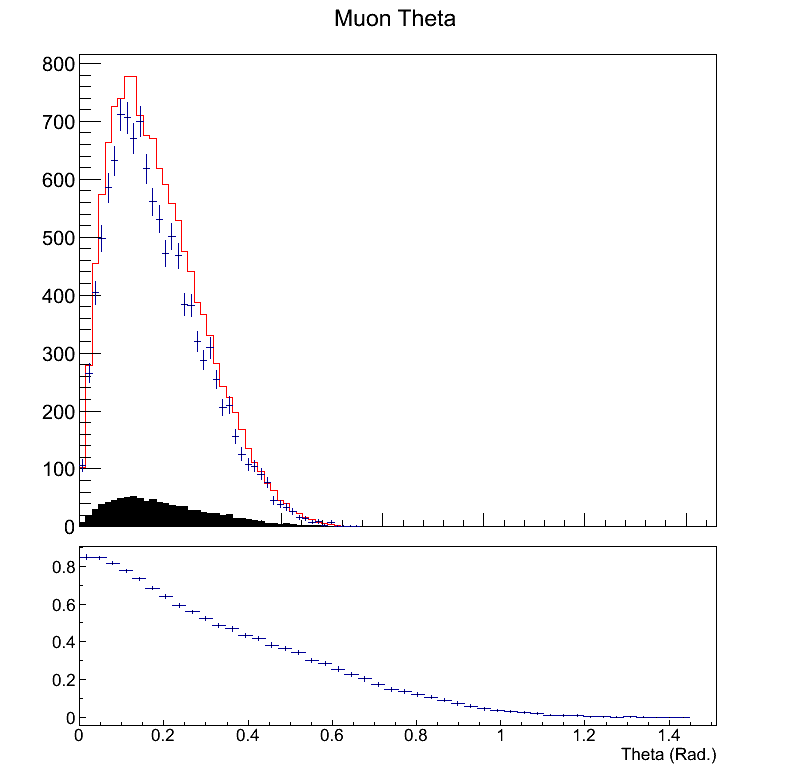
\includegraphics[width=3in]{Figures/TN100Plots/c_Thair_4.png}
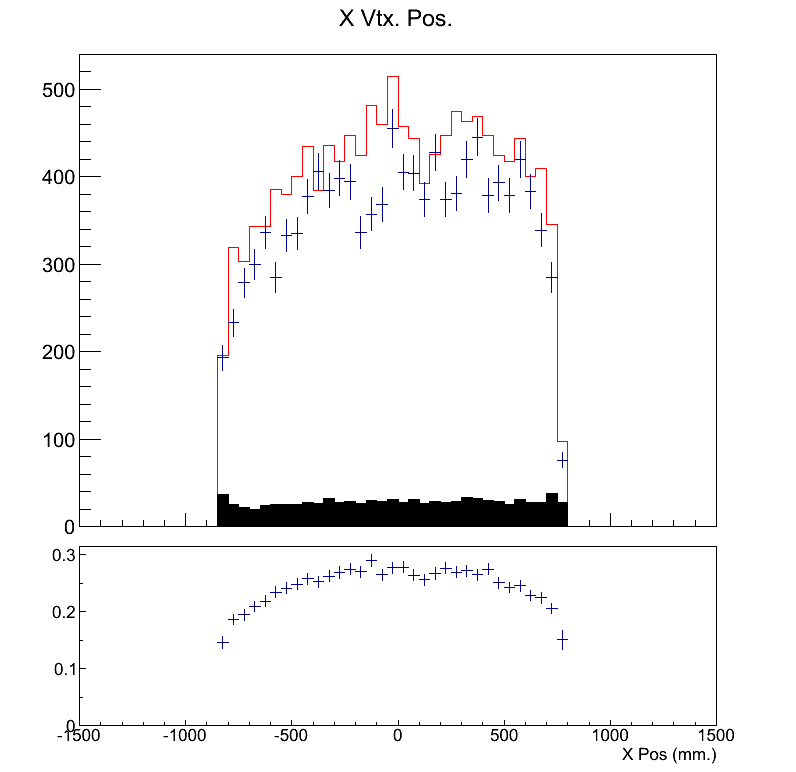
\includegraphics[width=3in]{Figures/TN100Plots/c_Xair_4.png}
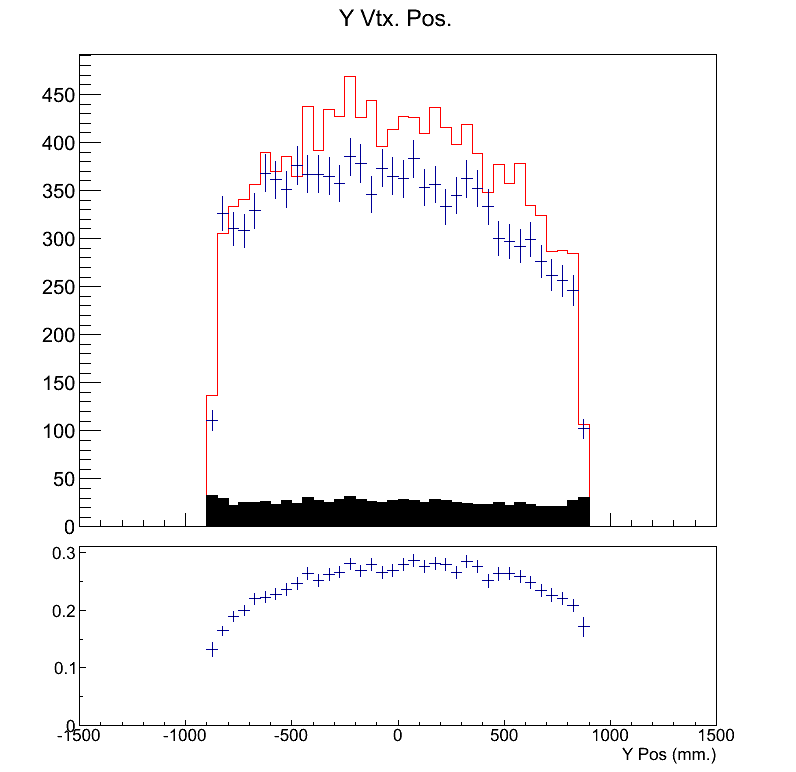
\includegraphics[width=3in]{Figures/TN100Plots/c_Yair_4.png}
\caption{Kinematic and Vertex position distributions for selected events in run 4 water-out. The data with error is shown with blue crosses and the MC signal and background are shown in red and black respectively. Below each distribution histogram is the MC predicted signal efficiency as a function of the same variable.}
\label{fig:xs2run4air}
\end{figure}

\begin{figure}[h]
\centering
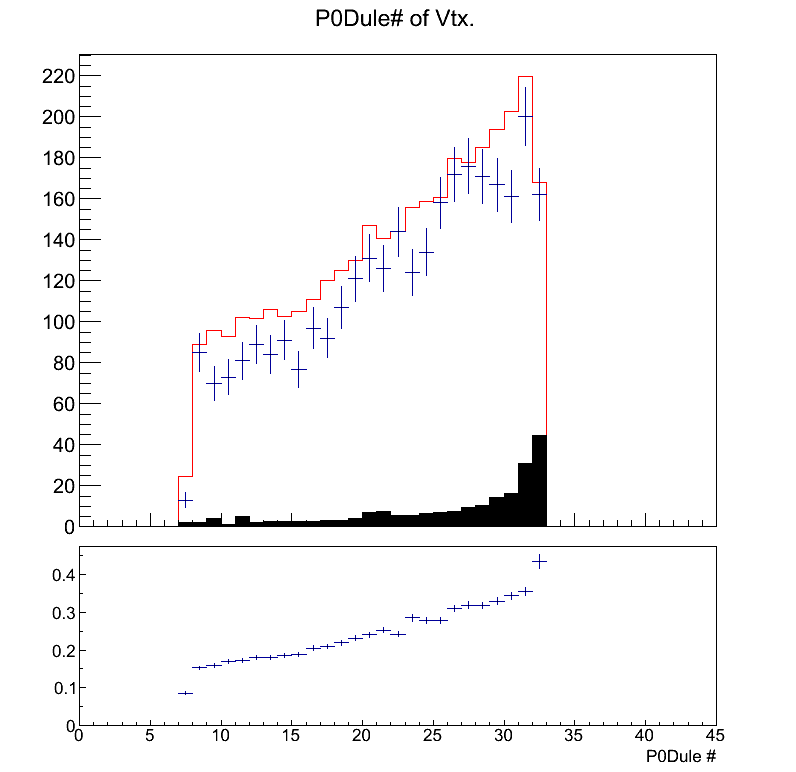
\includegraphics[width=2in]{Figures/TN100Plots/c_Layerwater_1.png}
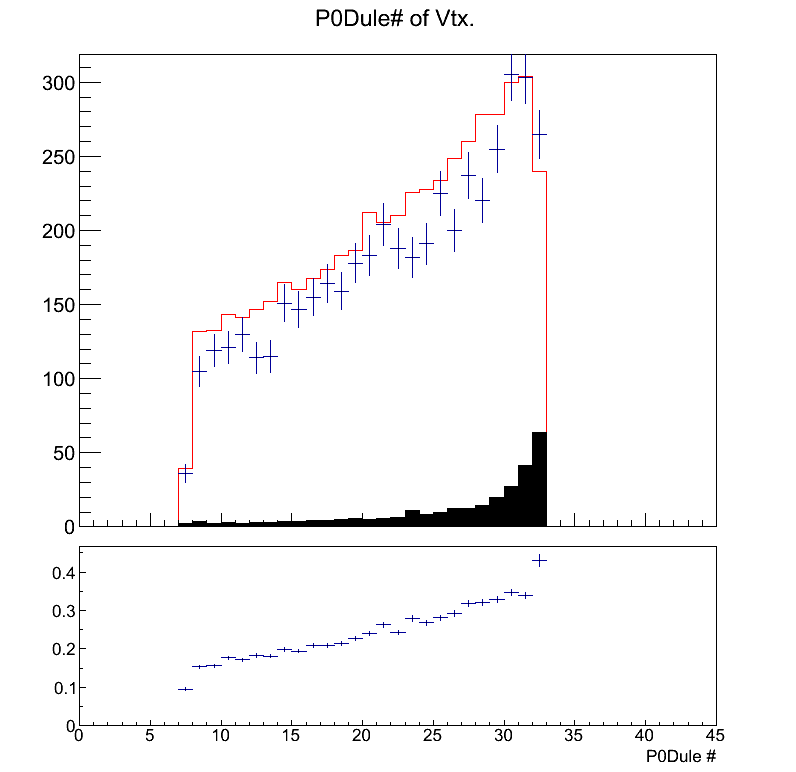
\includegraphics[width=2in]{Figures/TN100Plots/c_Layerwater_2.png}
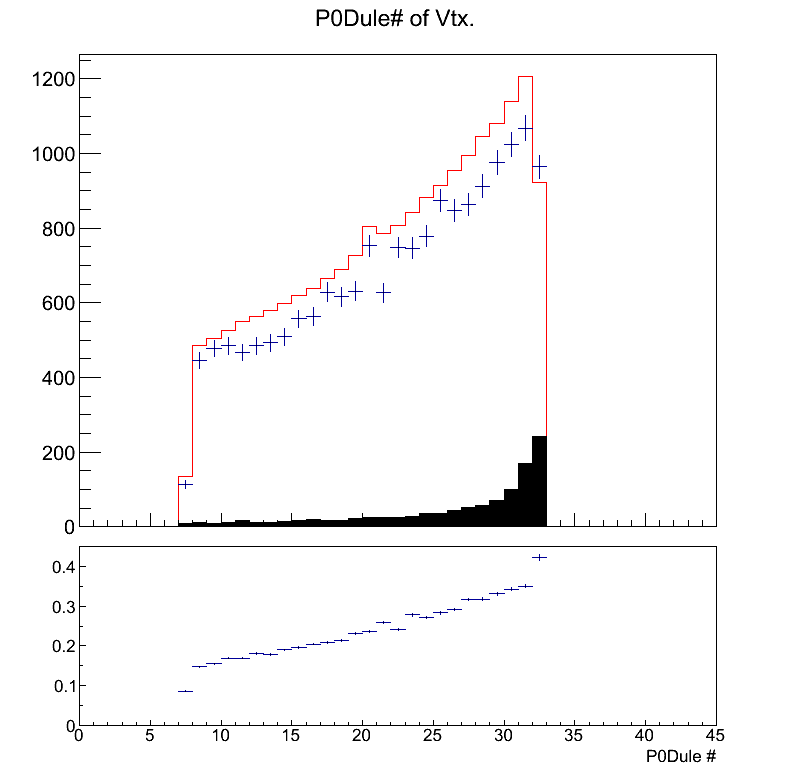
\includegraphics[width=2in]{Figures/TN100Plots/c_Layerwater_4.png}
\caption{The Z Vertex position distributions for selected events in water-in runs 1, 2 and 4 (left to right) binned by p0dule number. The data with error is shown with blue crosses and the MC signal and background are shown in red and black respectively. Below each distribution histogram is the MC predicted signal efficiency as a function of the same variable.}
\label{fig:xsZw}
\end{figure}

\begin{figure}[h]
\centering
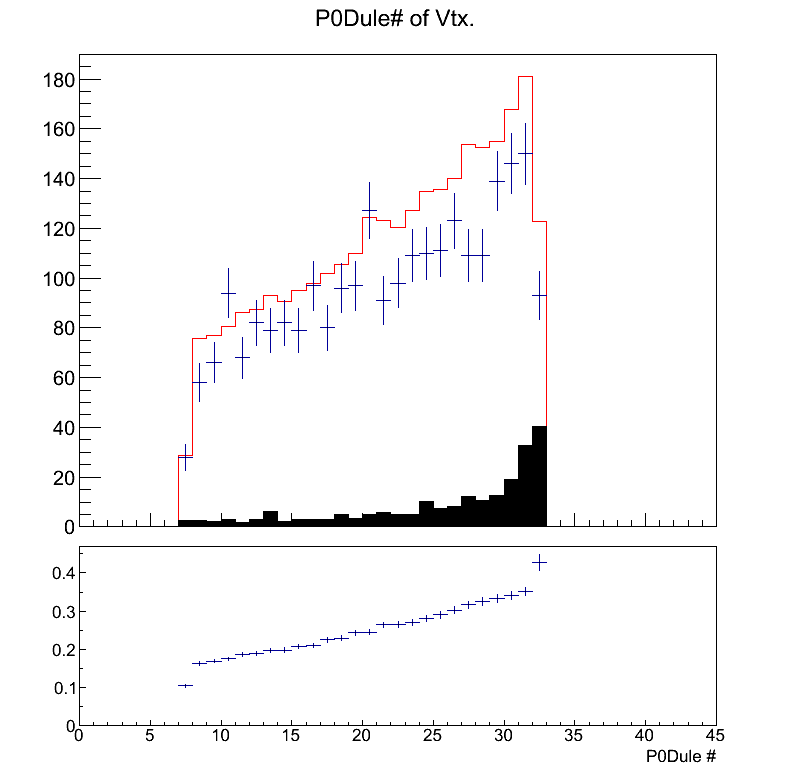
\includegraphics[width=2in]{Figures/TN100Plots/c_Layerair_2.png}
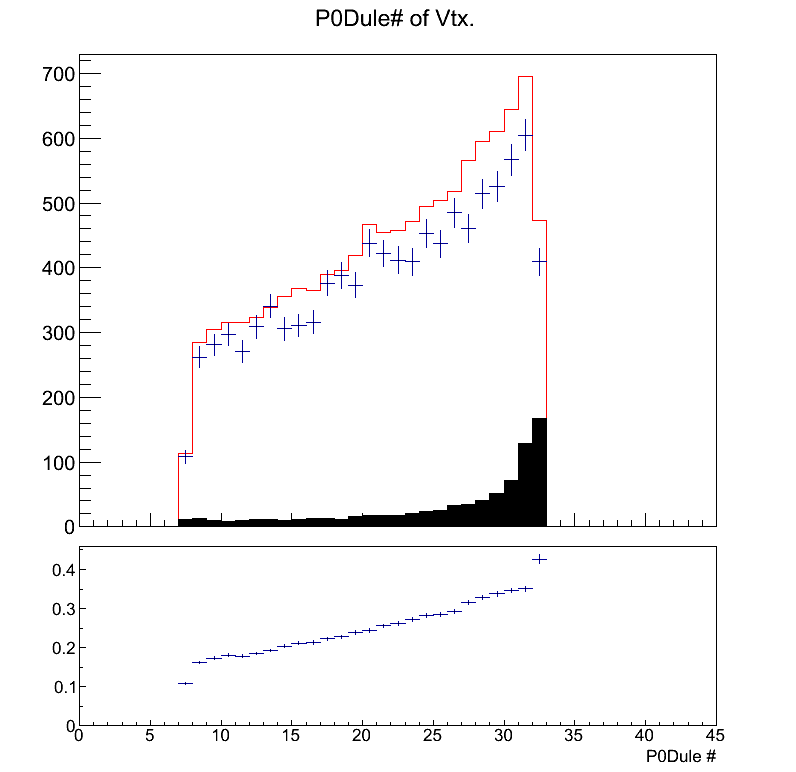
\includegraphics[width=2in]{Figures/TN100Plots/c_Layerair_3.png}
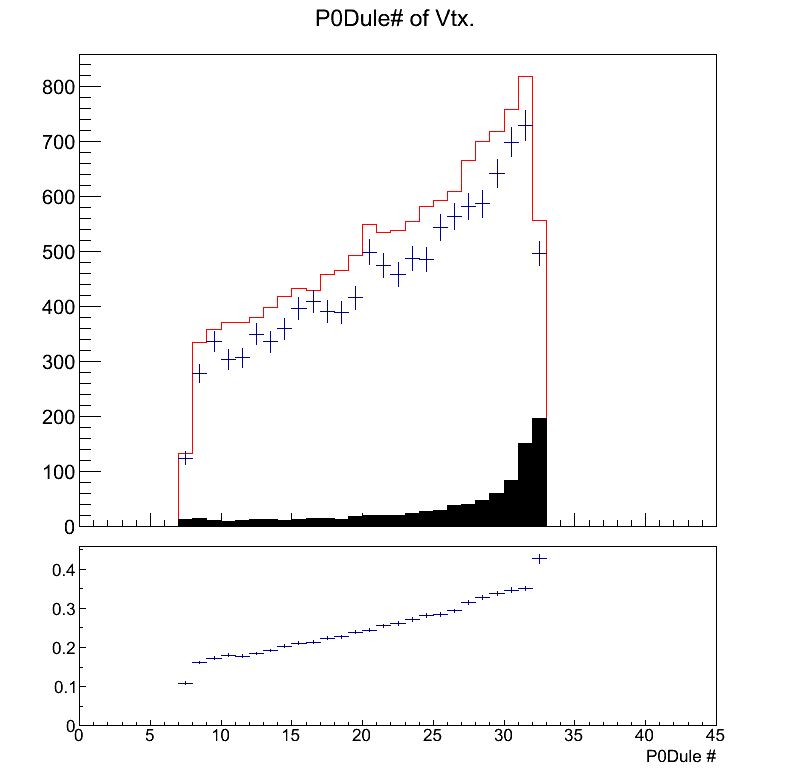
\includegraphics[width=2in]{Figures/TN100Plots/c_Layerair_4.png}
\caption{The Z Vertex position distributions for selected events in water-out runs 2, 3 and 4 (left to right) binned by p0dule number. The data with error is shown with blue crosses and the MC signal and background are shown in red and black respectively. Below each distribution histogram is the MC predicted signal efficiency as a function of the same variable.}
\label{fig:xsZa}
\end{figure}

The event yields for data and MC are given in Table \ref{tab:sel}. For an exposure of $23.47\times 10^{19}$ POT, we select 25,419 events in water-in data. For an exposure of $32.89\times 10^{19}$ POT, we select 24,250 events in water-out data. Figures \ref{fig:xsZw} and \ref{fig:xsZa} shows the Vertex distribution and signal efficiencies for water-in and water-out runs respectively. They are binned by P0dule number which is useful for the cross section extraction outlined later. The shape of the data and MC distributions agree, however the normalization to the data compared to the NEUT MC distributions are slightly lower.

\begin{table}[h]
\caption{The total selected events from each run. The MC is normalized by POT.}
\centering
\begin{tabular}{ccc} \toprule
 & Data & MC(norm.) \\
\hline
Run 1 water-in & 3106 & 3540 \\ 
Run 2 water-in & 4652 & 5149 \\ 
Run 2 water-out & 2521 & 2967.35 \\ 
Run 3 water-out & 10077 & 11239 \\ 
Run 4 water-in & 17661 & 19678 \\ 
Run 4 water-out & 11652 & 13223 \\ 
\hline
Total water-in & 25419 & 28366\\ 
Total water-out & 24250 & 27429\\ 
\bottomrule
\end{tabular} 
\label{tab:sel}
\end{table}